\section{Evaluation}

In this section,
we begin by evaluating \MSAGA{}'s performance compared to state-of-the-art systolic-array-based accelerators.
Then, we assess the accuracy impact of replacing \texttt{exp2} with PWL at the operator, kernel, and model levels.
Finally, we demonstrate \MSAGA{}'s minimal area overhead.

\subsection{\MSAGA{} Performance}\label{sec:eval-performance}

We compare the \FA{} performance of \MSAGA{} against state-of-the-art
systolic-array-based accelerators, 
including Google TPUv5e~\cite{gcp_tpuv5e} and AWS NeuronCore-v2~\cite{neuroncore-v2-arch}.
All accelerators use 16-bit floating-point activation 
and 32-bit accumulation, with the systolic array size of $128 \times 128$. 
\autoref{tab:accelerators-cfg} shows the detailed configurations.

We evaluate the forward pass performance of \FA{} using a single attention head 
on all accelerators. We use \FLOPs{} utilization as the performance metric, 
which reflects the end-to-end absolute performance of each accelerator 
under the same clock frequency, thereby eliminating the impact of 
frequency differences.
\FLOPs{} utilization is defined as:
\[
\text{\FLOPs{} Utilization} = 
\frac{\text{Achieved \FLOPs{}}}{\text{Peak \FLOPs{}}}
\]
where the achieved \FLOPs{} is calculated by:
\[
\text{Achieved \FLOPs{}} = 
\frac{\text{Total FLOPs}}{\text{Execution Time}}
\]
and the total number of FLOPs given by~\cite{fa2}:
\[
\text{Total FLOPs} = 4 \times \text{SeqLen}^2 \times d
\]
where $\text{SeqLen}$ is the sequence length and $d$ is the head dimension.

We use the official \FA{} kernel implementations for the two commercial 
accelerators, which are optimized for their respective architectures:
\begin{itemize}
  \item \textit{jax.experimental.pallas.ops.tpu.flash\_attention} for the TPUv5e~\cite{jax_pallas_tpu}.
  \item \textit{neuronxcc.nki.kernels.attention.flash\_fwd} for the AWS NeuronCore-v2~\cite{aws_neuron_nki}.
\end{itemize}
For \MSAGA{}, we use the \SA{} kernel as shown in \autoref{lst:msaga_fa_kernel}. 
In all experiments, we fix the head dimension at 128 and vary the sequence 
length from 2048 to 16384, without applying causal masking.


\begin{table}[t]
\centering
\begin{threeparttable}
\caption{Hardware configurations of accelerators.}
\label{tab:accelerators-cfg}
\begin{tabular}{cccc}
\toprule
\textbf{Accelerator}               & \textbf{TPUv5e}                          & \textbf{Neuron-v2}  & \textbf{\MSAGA{}}           \\
\midrule
Systolic array size       & $128$                         & $128$        & $128$         \\
Number of arrays & 4                               & 1              & 1               \\
\TFLOPs{} (MAC)     & 196.6                           & 91.75          & 32.77           \\
Frequency                 & 1.5GHz\tnote{1}                         & 2.8GHz         & 1.5GHz            \\
Memory Bandwidth          & 819GB/s                         & 820GB/s        & 820GB/s         \\
Scratchpad SRAM           & \multirow{2}{*}{48MiB} & 24MiB & 192KiB\tnote{2} \\
Accumulation SRAM         &                                 & 2MiB  & 64KiB  \\
Require Vector Unit?      & Yes                    & Yes   & No     \\
\bottomrule
\end{tabular}%
\begin{tablenotes}
  \footnotesize
  \item[1] The clock frequency of TPUv5e is inferred from its reported
  performance using this formula: $\text{freq}_{\text{GHz}} =
  \text{TFLOPS} \times 10^{12} / (2 \times 128 \times 128 \times 10^{9})$.
  \item[2] As \MSAGA{} operates on an $128 \times 128$ tile and only targets \FA{} operations in this experiment, 
  192\,KiB of SRAM is sufficient to support the algorithm.
\end{tablenotes}
\end{threeparttable}
\end{table}



\begin{figure}[t]
  \centering
  \ifreview
  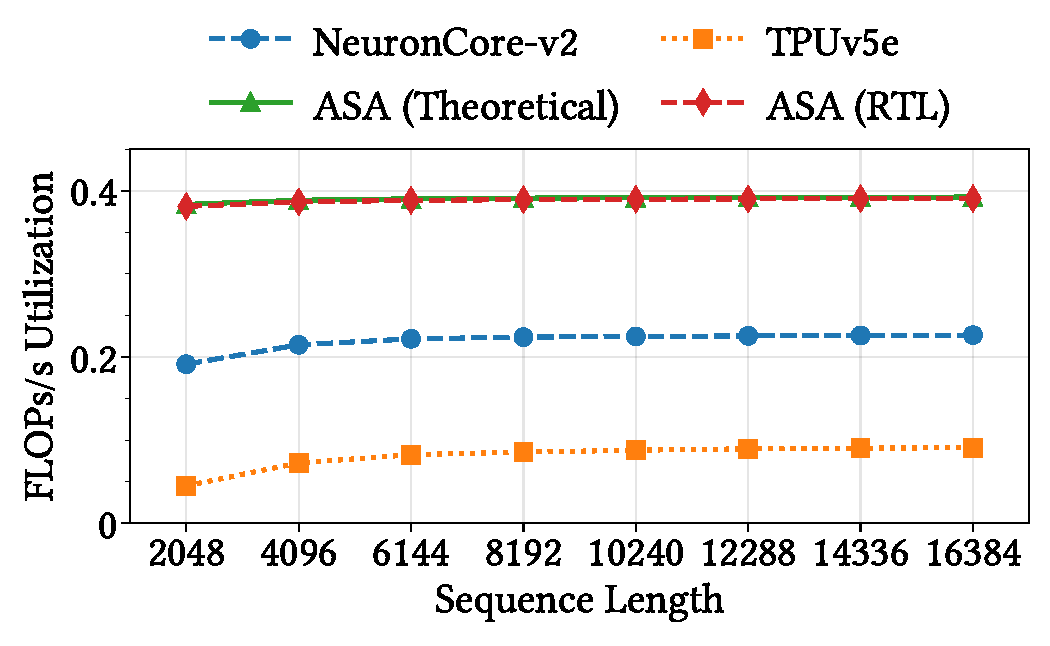
\includegraphics[width=1.0\columnwidth]{figure_src/perf.pdf}
  \else
  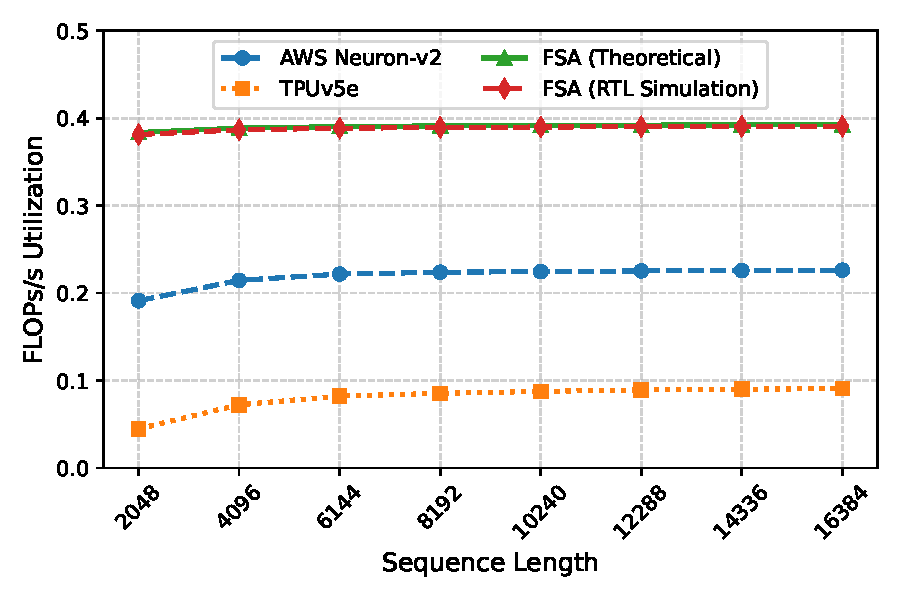
\includegraphics[width=1.0\columnwidth]{figure_src/perf_fsa.pdf}
  \fi
  \caption{\FA{} \FLOPs{} utilization of \MSAGA{} compared to TPUv5e and AWS NeuronCore-v2.}
  \label{fig:perf-cmp}
  \Description{
    The line plot shows the \FLOPs{} utilization of \MSAGA{} compared to TPUv5e and AWS NeuronCore-v2.
  }
\end{figure}

\autoref{fig:perf-cmp} shows the \FLOPs{} utilization of \MSAGA{}, TPUv5e and AWS NeuronCore-v2.
Benefiting from intensive operation overlapping, \MSAGA{} achieves \FLOPs{} utilization 1.77 times and 4.83 times higher
than those of TPUv5e and AWS NeuronCore-v2, respectively.
Moreover, the results confirm that our RTL 
implementation closely aligns with the theoretical performance 
outlined in \autoref{sec:overlapping-computations}, validating the 
correctness of our implementation.


\subsection{\MSAGA{} Accuracy}

The \SA{} produces mathematically equivalent results to standard attention with all orders of floating-point operations preserved. However, as PWL is used for the \texttt{exp2} computation, the final results may 
differ slightly from those generated by commercial accelerators.
In this section, we first analyze the accuracy of PWL 
approximation for the single \texttt{exp2} function. We then assess its overall 
impact on the final attention and model results.

\subsubsection{PWL Accuracy}

\begin{figure}[t]
  \centering
  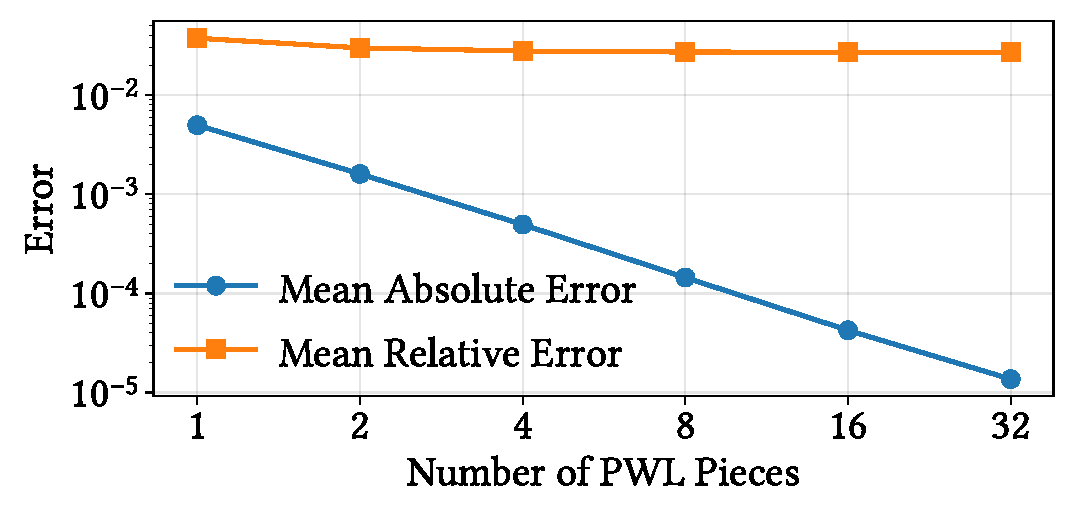
\includegraphics[width=\columnwidth]{figure_src/exp2.pdf}
  \caption{Mean absolute error (MAE) and mean relative error (MRE) of the piecewise linear approximation of \texttt{exp2}.}
  \label{fig:exp2-accuracy}
  \Description{}
\end{figure}

\begin{figure}[t]
  \centering
  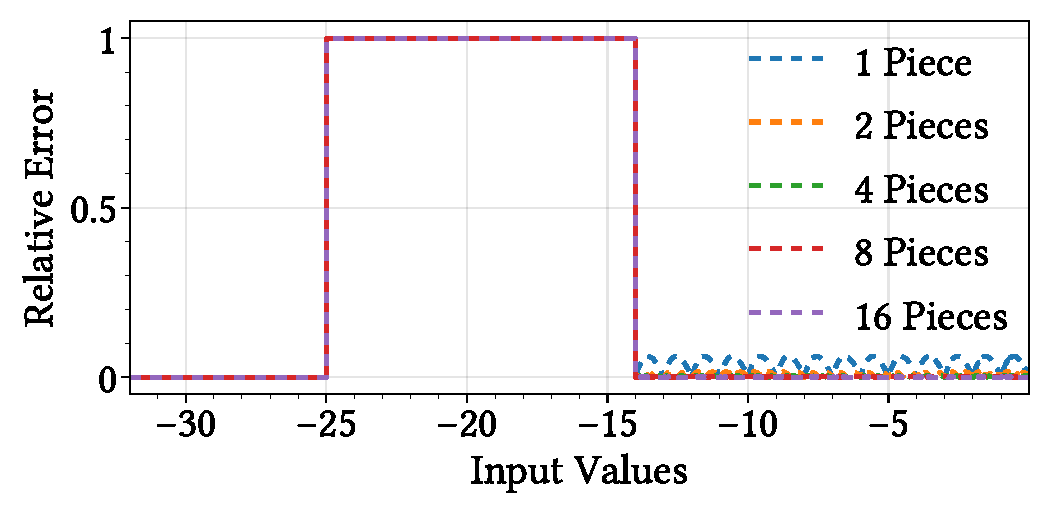
\includegraphics[width=\columnwidth]{figure_src/exp2_rel_err.pdf}
  \caption{\texttt{exp2} relative error distribution.}
  \label{fig:exp2-rel-distribution}
  \Description{
    The plot shows the mean absolute error (MAE) and mean relative error (MRE) 
    of the piecewise linear approximation of the softmax function as a function 
    of the number of pieces.
  }
\end{figure}

We exhaustively evaluate the PWL approximation over all negative 
\texttt{fp16} values as the input to the \texttt{exp2} function in \FA{} is always negative.
Subnormal values are excluded, as they are typically 
flushed to zero in most accelerators~\cite{googlebfloat16}.

\autoref{fig:exp2-accuracy} shows the mean absolute error (MAE) and 
mean relative error (MRE) of the PWL approximation of 
\texttt{exp2} with various numbers of pieces used. The MAE decreases 
significantly with more segments, while the MRE remains relatively stable. 
This behavior arises because the knots in PWL are 
uniformly spaced, whereas the \texttt{fp16} representation is logarithmic,
making the relative error more sensitive when output values 
are close to zero.

\autoref{fig:exp2-rel-distribution} shows the distribution of relative 
errors across input values. Most relative errors originate from the input 
range $[-25, -14]$, where the output of \texttt{exp2} is close to zero. 
Due to the limited precision of the piecewise approximation, the output 
often rounds to zero, leading to a relative error of 1.0.
For input values less than $-25$, both \texttt{exp2} and PWL output zero,
yielding a relative error of 0.
In our \MSAGA{} implementation, we use 8 segments, which achieves a 
MAE of 0.00014 and an MRE of 0.02728. Although non-uniformly spaced 
knots could reduce the MRE further, we leave this exploration 
to future work.

\subsubsection{\FA{} Accuracy}

We compare results from \SA{} against those from \textit{nn.functional.scaled\_dot\_\-product\_attention} in PyTorch~\cite{pytorch2} to evaluate \FA{} accuracy.
We use the same head dimension and sequence lengths as in the performance evaluation.
Following the same methodology of \FAthree{}~\cite{fa3}, we randomly generate input matrices using the following distribution:
\[
Q, K, V \sim \mathcal{N}(0, 1) + \mathcal{N}(0, 100) \cdot \mathrm{Bernoulli}(0.001).
\]

\begin{table}[t]
\centering
\caption{Mean absolute error (MAE), root mean squared error (RMSE), and mean relative error (MRE) of the \FA{} results on \MSAGA{}.}
\label{table:overall-accuracy}
\begin{tabular}{cccc}
\toprule
\textbf{SeqLen} & \textbf{MAE} & \textbf{RMSE} & \textbf{MRE} \\
\midrule
2048 & 7.983e-03 & 1.315e-02 & 1.558e-02 \\
4096 & 1.379e-02 & 2.290e-02 & 2.596e-02 \\
6144 & 1.849e-02 & 3.085e-02 & 3.545e-02 \\
8192 & 2.253e-02 & 3.772e-02 & 4.413e-02 \\
10240 & 2.595e-02 & 4.373e-02 & 5.259e-02 \\
12288 & 2.890e-02 & 4.873e-02 & 5.920e-02 \\
14336 & 3.165e-02 & 5.351e-02 & 6.529e-02 \\
16384 & 3.403e-02 & 5.784e-02 & 7.181e-02 \\
\bottomrule
\end{tabular}
\end{table}

The overall accuracy results are summarized in \autoref{table:overall-accuracy}.
Across all sequence lengths, MAE lies in the range from $7 \times 10^{-3}$ to $4 \times 10^{-2}$,
while MRE ranges from $1 \times 10^{-2}$ to $8 \times 10^{-2}$,
indicating that approximating \texttt{exp2} with PWL
has a negligible impact on the final attention result.

\subsubsection{End-to-End Model Accuracy}

\begin{table}[t]
\centering
\caption{Perplexity ($\downarrow$ lower is better) comparison between \FA{} 
with \texttt{exp2} and PWL approximations.}
\label{table:perplexity-comparison}
\begin{tabular}{cS[table-format=2.4]S[table-format=2.4]S[table-format=2.4]}
\toprule
\textbf{WikiText2 PPL $\downarrow$} & \textbf{FA-Exp2} & \textbf{FA-PWL} & \textbf{$\Delta$ PPL} \\
\midrule
Llama-3.2-1B & 12.9501 & 12.9492 & -0.0009 \\
Llama-3.2-3B & 10.2997 & 10.2998 & 0.0001 \\
Llama-3.1-8B & 8.1251 & 8.1254 & 0.0002 \\
Gemma-2-2B   & 11.5691 & 11.5680 & -0.0011 \\
Gemma-2-9B   & 9.0789  & 9.0780  & -0.0009 \\
Qwen2.5-0.5B & 19.6371 & 19.6387 & 0.0016 \\
Qwen2.5-1.5B & 13.3067 & 13.3086 & 0.0019 \\
Qwen2.5-3B   & 12.2867 & 12.2860 & -0.0007 \\
Qwen2.5-7B   & 9.5023  & 9.5027  & 0.0005 \\
Qwen2.5-14B  & 6.8394  & 6.8397  & 0.0002 \\
\bottomrule
\end{tabular}
\end{table}

To assess the impact of PWL on the model accuracy, we compare the word perplexity (PPL) of various models, including
Llama~\cite{llama3}, Gemma~\cite{gemma}, and Qwen~\cite{qwen25} families,
using the standard \texttt{exp2} and PWL respectively, with the 
WikiText2 dataset~\cite{wikitext2}.
Since even our largest FPGA cannot accommodate \MSAGA{} with the required $128 \times 128$ systolic array, we model PWL by replacing the \texttt{exp2f} function in the CUDA kernel of 
\FA{} with a software PWL implementation. 
As shown in \autoref{table:perplexity-comparison}, the perplexity with PWL remains almost identical to that of the original 
implementation, indicating that PWL has minimal impact on the performance of realistic LLM models.



\subsection{\MSAGA{} Area}\label{sec:area-overhead}


As described in \autoref{sec:msaga-design}, the area overhead of \MSAGA{} arises from the additional upward data path,
comparators, and Split units.
We synthesize \MSAGA{} systolic array (excluding SRAMs and DMA engines) at 1.5\,GHz using a commercial 16\,nm technology.
The breakdown of the total chip area into various components is shown in \autoref{tab:area}.
The standard systolic array occupies 87.92\% of the total area,
while \MSAGA{}'s additional components only contribute the remaining 12.07\%.
The dominant sources of area overhead come from the upward data path and Split units replicated for every PE,
accounting for 6.24\% and 5.30\% of the total area, respectively.
In contrast, the single array of comparators only consumes 0.53\% of the area.

\begin{table}[t]
\centering
\caption{\MSAGA{} area breakdown.}
\label{tab:area}
\begin{tabular}{@{}llrr@{}}
\toprule
\textbf{Group} & \textbf{Component}              & \textbf{Area (\%)}    & \textbf{Area ($\mu\mathrm{m}^2$)}   \\ \midrule
\multirow{3}{*}{Standard}
               & PEs      & 86.81                 & 24445044                            \\
               & Other logic                     & 1.11                  & 313457                              \\
               & \textit{Total}                  & 87.92                 & 24758501                            \\ \midrule
\multirow{4}{*}{\shortstack{\MSAGA{}\\additional}} 
               & Upward data path                & 6.24                  & 1756641                             \\
               & Split units                     & 5.30                  & 1493150                             \\
               & Comparators                     & 0.53                  & 149524                              \\
               & \textit{Total}                  & 12.07                 & 2029891                             \\ \bottomrule
\end{tabular}
\end{table}

